For each of the three different word embedding frameworks, one model, presented as the best performing for one framework in the previous chapter, is utilized to analyse the utility of the different linguistic features. This is done by expanding the input the model receives by the different feature groups of chapter \ref{feat_imp}.

\begin{figure}
    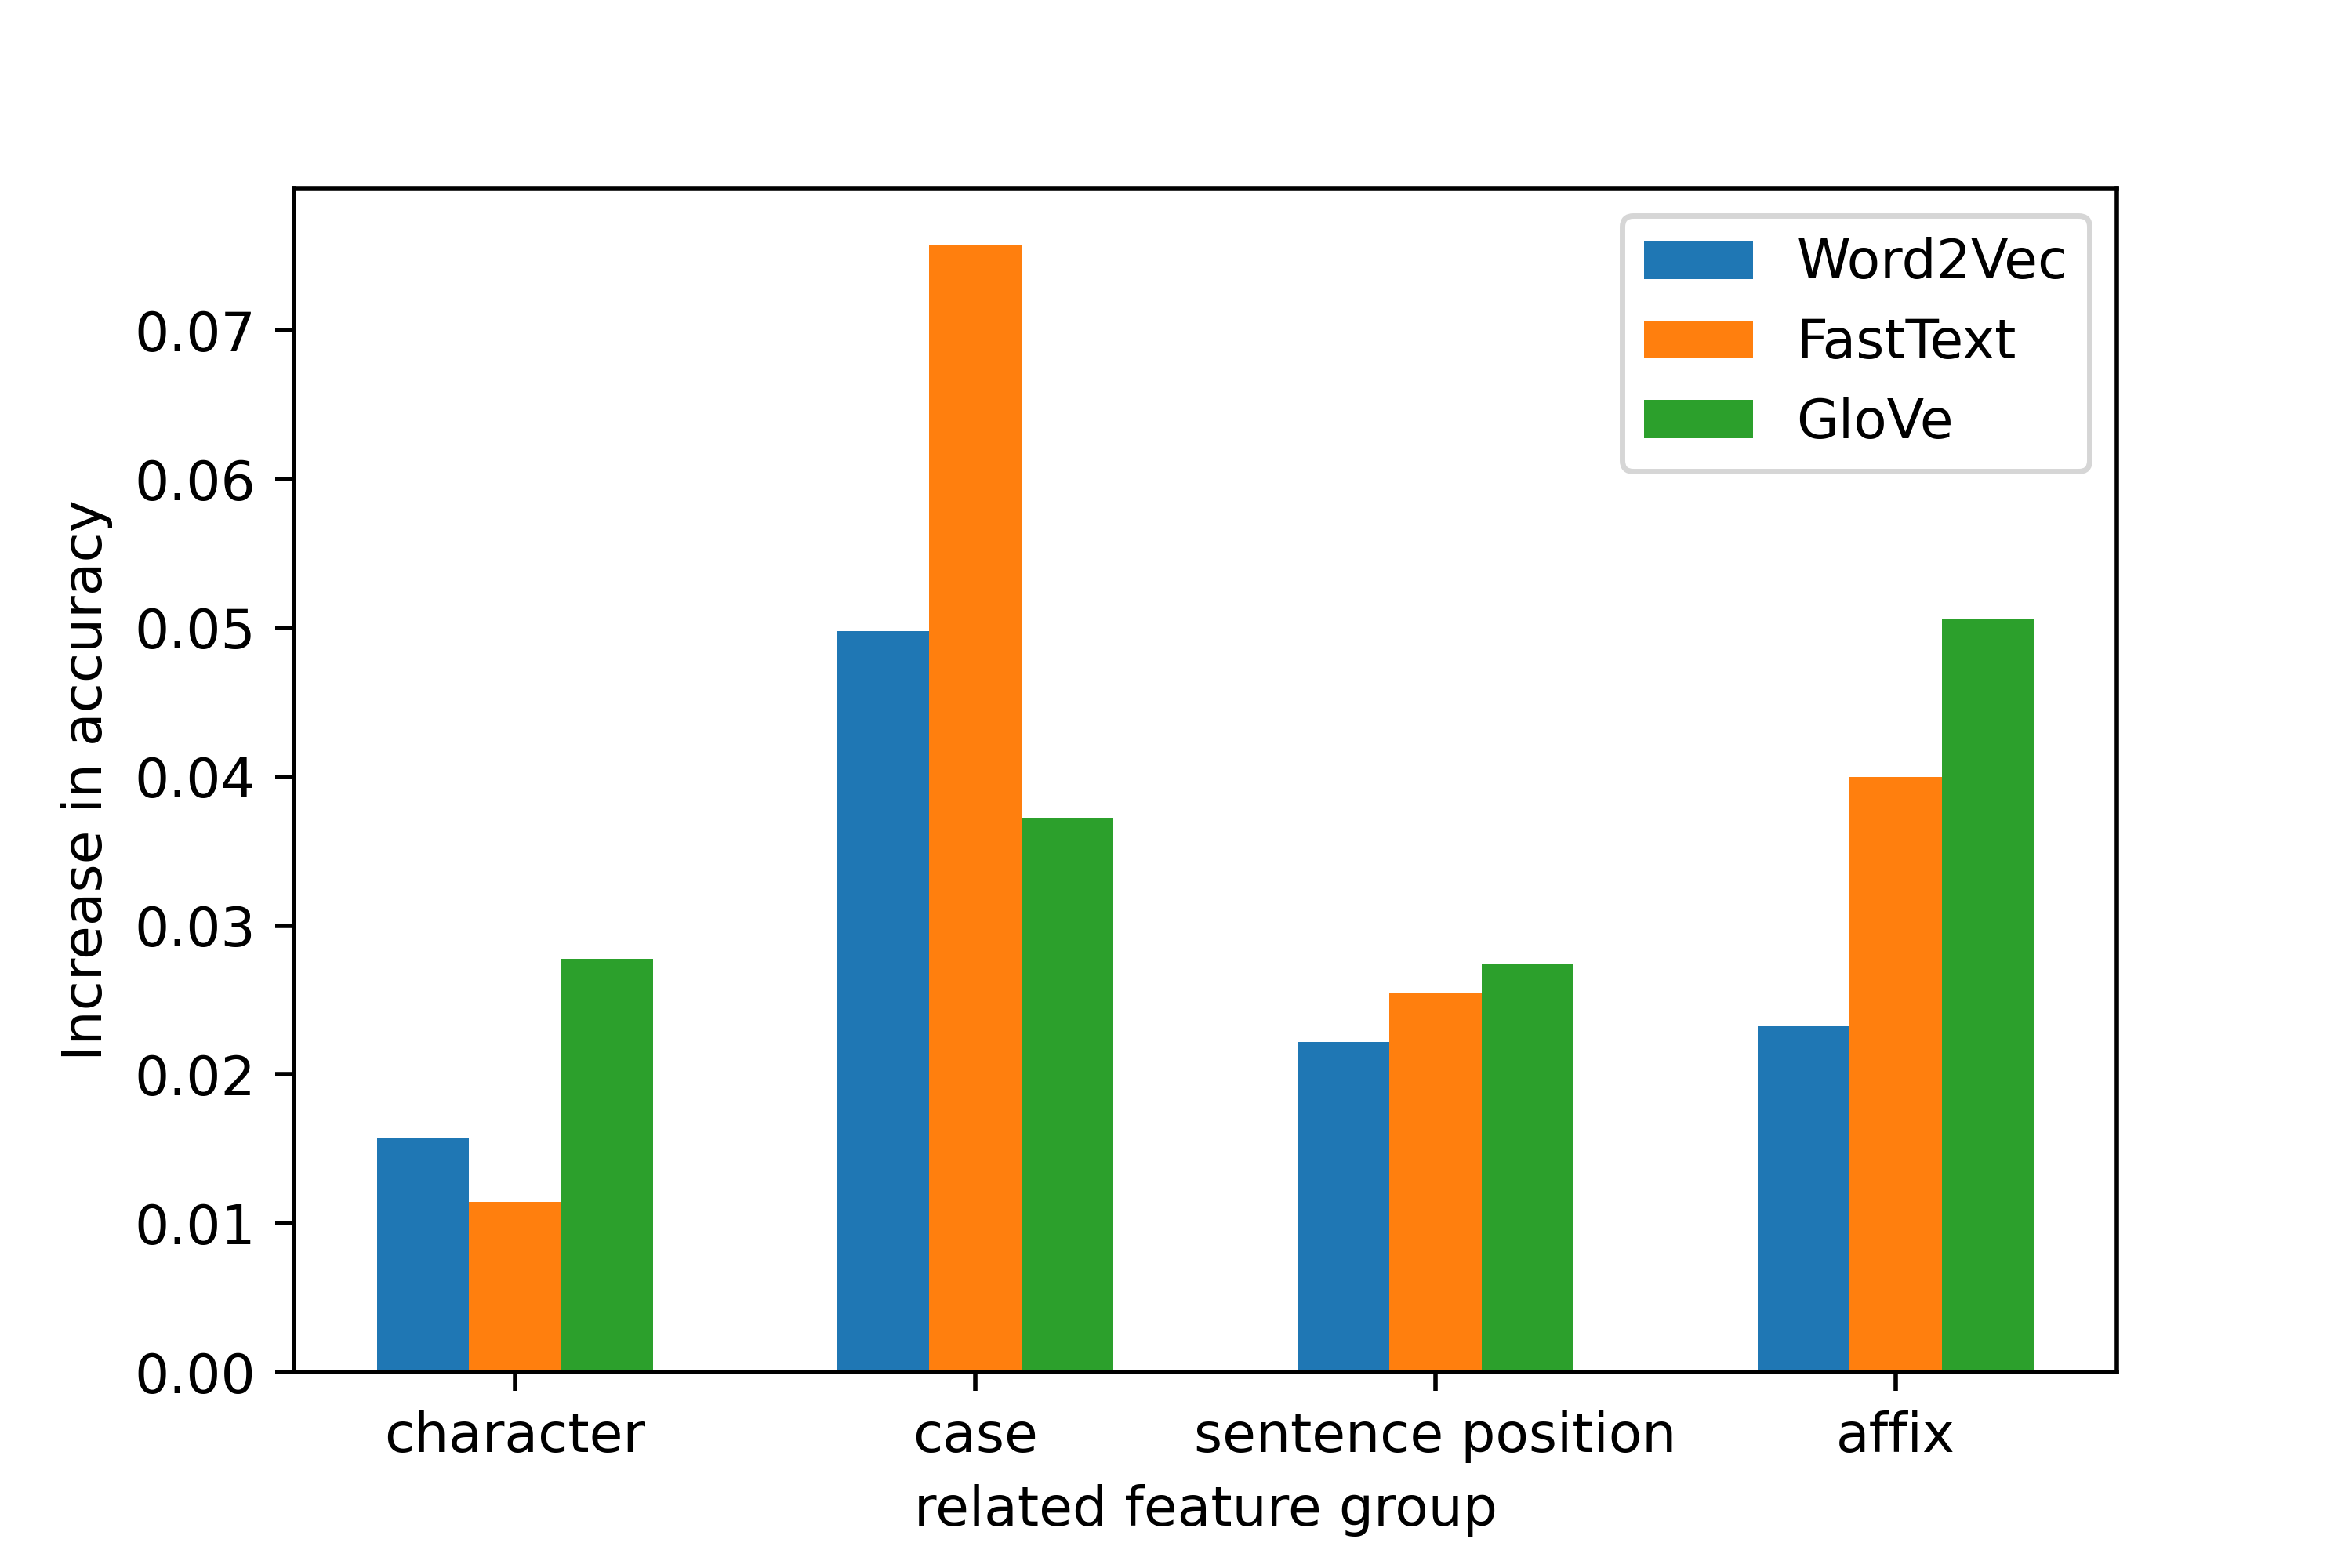
\includegraphics[width=\linewidth]{Pictures/accuracy_gain.png}
    \caption{Bar plot of the increase in accuracy of the POS-tagging model once one of the four feature groups is incorporated in the model in comparison to the model with the respective word embedding as its sole input.}
    \label{fig:acc}
\end{figure}


In figure \ref{fig:acc}, the gain in accuracy is depicted once a certain feature group is incorporated compared to the model with the word embedding as its sole input. It can be seen that the groups of character related and affix related features provide the biggest gain in accuracy for the POS-tagging models while the group of character related features is the least informative for the Word2Vec and FastText model.

\begin{table}[]
\centering
\begin{tabular}{|l|l|l|l|l|}
\thead{Framework} & \thead{related features} & \thead{accuracy} & \thead{weighted F1} & \thead{macro F1} \\
\hline
Word2Vec & character         & 0.0191 & 0.0235 & 0.0407 \\
Word2Vec & case              & 0.0528 & 0.0494 & 0.0480 \\
Word2Vec & sentence position & 0.0268 & 0.0340 & 0.0435 \\
Word2Vec & affix             & 0.0500 & 0.0614 & 0.0495 \\ \hline
FastText & character         & 0.0102 & 0.0143 & 0.0223 \\
FastText & case              & 0.0646 & 0.0614 & 0.0611 \\
FastText & sentence position & 0.0294 & 0.0343 & 0.0435 \\
FastText & affix             & 0.0368 & 0.0468 & 0.0402 \\ \hline
GloVe    & character         & 0.0079 & 0.0080 & 0.0094 \\
GloVe    & case              & 0.0219 & 0.0228 & 0.0255 \\
GloVe    & sentence position & 0.0157 & 0.0176 & 0.0242 \\
GloVe    & affix             & 0.0332 & 0.0360 & 0.0270 \\ \hline
\end{tabular}
\caption{Average increase in the metrics accuracy, weighted F1-score and macro F1-score once a feature group is added compared to each model that does not incorporate that feature group.}
\label{tab:feat_group}
\end{table}


Table \ref{tab:feat_group} shows the change in model performance on the POS-tagging task once a certain feature group is included in the LSTM Neural Network compared to the model without the information of this feature group. 

The values are obtained by averaging the distance in the metrics between models that incorporate that feature group and ones that do not while being exactly similar in all other aspects. 
For the POS-tagging models with the self-trained word embeddings, utilizing the group of case related features results in biggest increase in all but one of the depicted evaluation metrics. 

For models with the GloVe word embedding, the incorporation of the group of affix related features produces the biggest increase in the evaluation metrics. This may have been due to a incapability of the GloVe framework to capture meaningful sub-word level information while being high quality word embeddings in general (since the embedddings were pre-trained on huge amounts of data).

Word2Vec models have a bigger increase in the metrics if the affix feature group is utilized compared to the FastText models which could indicate that the FastText framework was able to capture meaningful sub-word level information regarding affixes on itself.

The performance of the POS-tagging models on the level of individual tags varies strongly, but the tendency that tags that occur seldom in general are mostly ignored can be shown by the fact that for the tag 'X' which has occurred only 252 times in the training data all POS-tagging models have a F1-score of 0 for this tag.

No meaningful change in model performance was perceived by changing the word embedding position from the beginning of the input space to its end.

Overall, the combinations of feature groups, the word embedding position and the three frameworks for word embeddings resulted in 93 POS-tagging models that were evaluated with the before mentioned metrics. The best perfoming POS-tagging model was a LSTM Neural Network with 125 units in its hidden layer, the GloVe word embedding with vector size 200 and all feature groups as its input. It has achieved an accuracy of 0.882 and a weighted F1-score of 0.877.

As a baseline for putting the evaluated models in perspective, a tagger was build that assigns the most common tag for a word in the training data to each respective word that was encountered and the the most common tag in general ('NOUN') to before unseen words. This baseline tagger has achieved an accuracy of 0.828 on the POS-tagging task on the GUM data. 26 of the 93 thoroughly investigated LSTM Neural Networks have performed on this task with a higher accuracy. 24 of them incorporated the pretrained GloVe word embeddings while two of them used the self-trained Word2Vec word embeddings.
